\chapter{Fabrication of Depletion-Mode HEMT Devices}

\section{Overview of the Fabrication Workflow}

The depletion--mode HEMTs characterised in this report were fabricated
using the standard III--V device process established within the Leeds
Nanotechnology Cleanroom. The workflow follows the routine sequence used
for GaAs/AlGaAs transistors in this facility, comprising mesa definition,
ohmic contact formation, contact annealing and Schottky--gate
metallisation. This well-established procedure was followed without
modification and carried out over four full-day laboratory sessions. The devices
produced through this workflow provide a reliable baseline against which
the behaviour of devices with different structures and dimensions can be compared.

\vspace{3mm}

% FIGURE: Cleanroom process overview (optional)


\section{Mesa Definition and Isolation Etch}

The fabrication process began with the electrical isolation of individual device
regions through mesa etching. Prior to lithography, the GaAs wafer was
cleaned sequentially in acetone, isopropanol (IPA) and deionised water (DI) to
remove organic residues and ensure good photoresist adhesion. A positive
 photoresist (S1803) was then spun onto the sample at 3000rpm, soft-baked at
 approximately 115\,$^{\circ}$C, and then patterned with exposure from the Heidelberg MLA 150 
 - Maskless Aligner (MLA).

\vspace{2mm}
\begin{figure}[htbp]
  \centering
  \includegraphics[width=0.5\linewidth]{figures/fabrication_images/mesa_mask.jpg}
  \caption{Mesa lithography mask used for defining isolated device regions. (Post-Development)}
  \label{fig:mesa_mask}
\end{figure}

Following development, the mesa pattern was transferred into the wafer using a sulphuric
acid, hydrogen peroxide and water wet-etch solution (160:8:1 ratio). This etchant is well suited
to GaAs/AlGaAs mesa formation because it produces a controllable, moderately fast isotropic
etch (typically a few nanometres per second) that removes the active layers uniformly. Its rate is
slow enough to time accurately for a shallow $\approx 200\,\text{nm}$ recess, yet fast enough to
be practical for routine device isolation.

\vspace{2mm}

To calibrate the process, a 30\,s pilot etch was performed, and the depth measured using the
Alpha-Step profilometer, giving an initial etch rate of approximately $3.8\,\text{nm\,s}^{-1}$.
Using this value, the main mesa etch was timed to reach the target recess. During the second
etch, the measured rate decreased to around $2.9\,\text{nm\,s}^{-1}$, most likely due to cooling of
the etchant after mixing. Since the reaction rate of this chemistry is temperature dependent, a
lower solution temperature reduces its reactivity and therefore slows the etch.

\vspace{2mm}

This variation highlighted the sensitivity of the process to temperature and timing. For
future wet-etching, the etchant temperature will be monitored before and during
etching, and the solution will be used promptly after mixing to ensure consistent reactivity.

\vspace{3mm}

\section{Ohmic Contact Formation}

When a metal is deposited directly onto the GaAs cap, the interface would naturally forms a Schottky
barrier, which behaves like a diode and restricts carrier injection into the channel. Ohmic
contacts are used to avoid this; during annealing the AuGe layer alloys with the GaAs and
creates a heavily doped region beneath the metal, thinning the barrier sufficiently for current to
enter the 2DEG with low resistance.

\vspace{2mm}

To pattern these contacts cleanly, a dual-layer photoresist stack of LOR beneath S1803 was used.
A single photoresist layer develops near-vertical sidewalls, causing the evaporated metal to form a
continuous film across both the wafer surface and the photoresist edges. This continuity makes lift-off
unreliable and often leaves metallic flakes or fences around the contact perimeter.

\vspace{2mm}

The dual-layer stack overcomes this by exploiting the higher developer solubility of LOR.
During development, the LOR recedes laterally more than the S1803 above it, producing the
undercut profile shown in Figure~3.2. This undercut breaks the continuity of the deposited
metal so the film on top of the photoresist is physically separated from the metal inside the opening.
When the layers of photoresist dissolve during lift-off, the unwanted metal lifts away cleanly, leaving sharply
defined contact openings ready for metallisation.

\vspace{2mm}

% Dual-layer resist stack showing undercut for clean lift-off
\begin{figure}[htbp]
  \centering
  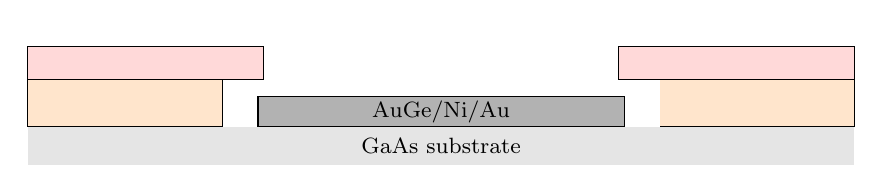
\begin{tikzpicture}[x=1.5cm,y=0.6cm,font=\footnotesize]
    % Dimensions
    \def\w{7}
    \def\hsub{0.8}
    \def\hlor{1.0}
    \def\hs1803{0.7}
    \def\gap{0.35}
    \def\xL{2.0}
    \def\xR{5.0}

    % Keep bounding box tight to the main drawing so labels don't shift centering
    \path[use as bounding box] (0,0) rectangle (\w,\hsub+\hlor+\hs1803+0.4);

    % Substrate (GaAs)
    \fill[gray!20] (0,0) rectangle (\w,\hsub);
    \node at (3.5,0.4) {GaAs substrate};

    % LOR with wider opening (split to avoid outlines across the gap)
    \fill[orange!20] (0,\hsub) rectangle (\xL-\gap,\hsub+\hlor);
    \draw (0,\hsub) rectangle (\xL-\gap,\hsub+\hlor);
    \fill[orange!20] (\xR+\gap,\hsub) rectangle (\w,\hsub+\hlor);
    \draw (\xR+\gap,\hsub) rectangle (\w,\hsub+\hlor);

    % Remove opening in LOR (undercut wider)
    \fill[white] (\xL-\gap,\hsub) rectangle (\xR+\gap,\hsub+\hlor);
    \node[anchor=east] at (-0.2,\hsub+0.5*\hlor) {LOR (undercut)};

    % S1803 with narrower opening (split to avoid outlines across the gap)
    \fill[red!15] (0,\hsub+\hlor) rectangle (\xL,\hsub+\hlor+\hs1803);
    \draw (0,\hsub+\hlor) rectangle (\xL,\hsub+\hlor+\hs1803);
    \fill[red!15] (\xR,\hsub+\hlor) rectangle (\w,\hsub+\hlor+\hs1803);
    \draw (\xR,\hsub+\hlor) rectangle (\w,\hsub+\hlor+\hs1803);
    \fill[white] (\xL,\hsub+\hlor) rectangle (\xR,\hsub+\hlor+\hs1803);
    \node[anchor=east] at (-0.2,\hsub+\hlor+0.5*\hs1803) {S1803};

    % Metal deposition (wider, under the S1803 opening)
    \fill[gray!60] (\xL-0.05,\hsub) rectangle (\xR+0.05,\hsub+0.65);
    \draw (\xL+-0.05,\hsub) rectangle (\xR+0.05,\hsub+0.65);
    \node at (3.5,\hsub+0.32) {AuGe/Ni/Au};

  \end{tikzpicture}
  \caption{Dual-layer LOR/S1803 resist stack after development showing the wider LOR opening that creates an undercut for clean metal lift-off.}
  \label{fig:lift_off_stack}
\end{figure}


\vspace{2mm}

A AuGe/Ni/Au metallisation stack was then deposited via thermal evaporation to form the
ohmic contacts. During the subsequent anneal the AuGe alloys with the GaAs to create the
heavily doped contact region required for a linear, low-resistance interface. After deposition,
solvent-based lift-off removed the excess metal, leaving well defined pads with smooth edges
and good adhesion, as shown in Figure~\ref{fig:ohmic_contacts}.

\vspace{3mm}

\begin{figure}[htbp]
    \centering
    \includegraphics[width=0.5\linewidth]{figures/fabrication_images/ohmic_formation.jpg}
    \caption{Ohmic contacts after lift-off.}
    \label{fig:ohmic_contacts}  
\end{figure}


\section{Contact Annealing, Gate Formation and Final Inspection}

The sample was annealed to activate the AuGe/Ni/Au contacts and form a
low-resistance alloyed interface with the GaAs surface. During annealing
germanium diffuses into the GaAs, locally increasing the doping
concentration beneath the contacts and thereby reducing the contact
resistance.

\vspace{2mm}

With the ohmic contacts established, a third photolithography step defined
the gate region. As before, a dual-layer resist stack was used to ensure
reliable lift-off. The gate electrode was aligned centrally between the
source and drain to modulate the 2DEG formed at the AlGaAs/GaAs
interface. Following development, Ti/Au was evaporated to form the
Schottky gate metal stack, with titanium acting as an adhesion layer and
gold providing a stable Schottky barrier and a low-resistance gate
conductor.

\vspace{2mm}

\begin{figure}[htbp]
    \centering
    \includegraphics[width=0.5\linewidth]{figures/fabrication_images/gold_formation_zoomed.jpg}
    \caption{Gate contacts after lift-off.}
    \label{fig:gate_contacts}  
\end{figure}

\vspace{3mm}

After gate metallisation, the resist was removed using solvent lift-off,
revealing the final device structure. A small number of lift-off
defects, primarily isolated metallic particles, were observed under the
microscope and removed using brief, gentle ultrasonic cleaning. These
artefacts can cause electrical short circuits, particularly around the
gate edges, so their removal was essential for device reliability.

\vspace{2mm}

The completed devices were examined using optical microscopy. The mesas
exhibited clean sidewalls, the ohmic pads were well defined, and the
gate electrodes showed sharp, uninterrupted edges with no bridging or
residual flakes. Overall, the process yielded a high-quality array of
depletion-mode HEMTs suitable for subsequent electrical characterisation.


